\documentclass[a4paper,11pt,fleqn,twoside,openright]{memoir} 	% Openright aabner kapitler paa hoejresider (openany begge)

%%%% PACKAGES %%%%

% ¤¤ Oversaettelse og tegnsaetning ¤¤ %
\usepackage[utf8]{inputenc}					% Input-indkodning af tegnsaet (UTF8)
\usepackage[danish]{babel}					% Dokumentets sprog
\usepackage[T1]{fontenc}					% Output-indkodning af tegnsaet (T1)
\usepackage{ragged2e,anyfontsize}			% Justering af elementer
\usepackage{fixltx2e}						% Retter forskellige fejl i LaTeX-kernen
																			
% ¤¤ Figurer og tabeller (floats) ¤¤ %
\usepackage{graphicx} 						% Haandtering af eksterne billeder (JPG, PNG, PDF)
\usepackage{multirow}                		% Fletning af raekker og kolonner (\multicolumn og \multirow)
\usepackage{colortbl} 						% Farver i tabeller (fx \columncolor, \rowcolor og \cellcolor)
\usepackage[dvipsnames]{xcolor}				% Definer farver med \definecolor. Se mere: http://en.wikibooks.org/wiki/LaTeX/Colors
\usepackage{flafter}						% Soerger for at floats ikke optraeder i teksten foer deres reference
\let\newfloat\relax 						% Justering mellem float-pakken og memoir
\usepackage{float}							% Muliggoer eksakt placering af floats, f.eks. \begin{figure}[H]
%\usepackage{eso-pic}						% Tilfoej billedekommandoer paa hver side
%\usepackage{wrapfig}						% Indsaettelse af figurer omsvoebt af tekst. \begin{wrapfigure}{Placering}{Stoerrelse}
%\usepackage{multicol}         	        	% Muliggoer tekst i spalter
%\usepackage{rotating}						% Rotation af tekst med \begin{sideways}...\end{sideways}

% ¤¤ Matematik mm. ¤¤
\usepackage{amsmath,amssymb,stmaryrd} 		% Avancerede matematik-udvidelser
\usepackage{mathtools}						% Andre matematik- og tegnudvidelser
\usepackage{textcomp}                 		% Symbol-udvidelser (f.eks. promille-tegn med \textperthousand )
\usepackage{siunitx}						% Flot og konsistent praesentation af tal og enheder med \si{enhed} og \SI{tal}{enhed}
\sisetup{output-decimal-marker = {,}}		% Opsaetning af \SI (DE for komma som decimalseparator) 
\usepackage[version=3]{mhchem} 				% Kemi-pakke til flot og let notation af formler, f.eks. \ce{Fe2O3}
%\usepackage{rsphrase}						% Kemi-pakke til RS-saetninger, f.eks. \rsphrase{R1}

% ¤¤ Referencer og kilder ¤¤ %
\usepackage[danish]{varioref}				% Muliggoer bl.a. krydshenvisninger med sidetal (\vref)
\usepackage{natbib}							% Udvidelse med naturvidenskabelige citationsmodeller
%\usepackage{xr}							% Referencer til eksternt dokument med \externaldocument{<NAVN>}
%\usepackage{glossaries}					% Terminologi- eller symbolliste (se mere i Daleifs Latex-bog)

% ¤¤ Misc. ¤¤ %
\usepackage{listings}						% Placer kildekode i dokumentet med \begin{lstlisting}...\end{lstlisting}
\usepackage{lipsum}							% Dummy text \lipsum[..]
\usepackage[shortlabels]{enumitem}			% Muliggoer enkelt konfiguration af lister
\usepackage{pdfpages}						% Goer det muligt at inkludere pdf-dokumenter med kommandoen \includepdf[pages={x-y}]{fil.pdf}	
\pdfoptionpdfminorversion=6					% Muliggoer inkludering af pdf dokumenter, af version 1.6 og hoejere
\pretolerance=2500 							% Justering af afstand mellem ord (hoejt tal, mindre orddeling og mere luft mellem ord)

% Kommentarer og rettelser med \fxnote. Med 'final' i stedet for 'draft' udloeser hver note en error i den faerdige rapport.
\usepackage[footnote,draft,danish,silent,nomargin]{fixme}		


%%%% CUSTOM SETTINGS %%%%

% ¤¤ Marginer ¤¤ %
\setlrmarginsandblock{3.5cm}{2.5cm}{*}		% \setlrmarginsandblock{Indbinding}{Kant}{Ratio}
\setulmarginsandblock{2.5cm}{3.0cm}{*}		% \setulmarginsandblock{Top}{Bund}{Ratio}
\checkandfixthelayout 						% Oversaetter vaerdier til brug for andre pakker

%	¤¤ Afsnitsformatering ¤¤ %
\setlength{\parindent}{0mm}           		% Stoerrelse af indryk
\setlength{\parskip}{3mm}          			% Afstand mellem afsnit ved brug af double Enter
\linespread{1,1}							% Linie afstand

% ¤¤ Litteraturlisten ¤¤ %
\bibpunct[,]{[}{]}{;}{a}{,}{,} 				% Definerer de 6 parametre ved Harvard henvisning (bl.a. parantestype og seperatortegn)
\bibliographystyle{bibtex/harvard}			% Udseende af litteraturlisten.

% ¤¤ Indholdsfortegnelse ¤¤ %
\setsecnumdepth{subsection}		 			% Dybden af nummerede overkrifter (part/chapter/section/subsection)
\maxsecnumdepth{subsection}					% Dokumentklassens graense for nummereringsdybde
\settocdepth{subsection} 					% Dybden af indholdsfortegnelsen

% ¤¤ Lister ¤¤ %
\setlist{
  topsep=0pt,								% Vertikal afstand mellem tekst og listen
  itemsep=-1ex,								% Vertikal afstand mellem items
} 

% ¤¤ Visuelle referencer ¤¤ %
\usepackage[colorlinks]{hyperref}			% Danner klikbare referencer (hyperlinks) i dokumentet.
\hypersetup{colorlinks = true,				% Opsaetning af farvede hyperlinks (interne links, citeringer og URL)
    linkcolor = black,
    citecolor = black,
    urlcolor = black
}

% ¤¤ Opsaetning af figur- og tabeltekst ¤¤ %
\captionnamefont{\small\bfseries\itshape}	% Opsaetning af tekstdelen ('Figur' eller 'Tabel')
\captiontitlefont{\small}					% Opsaetning af nummerering
\captiondelim{. }							% Seperator mellem nummerering og figurtekst
\hangcaption								% Venstrejusterer flere-liniers figurtekst under hinanden
\captionwidth{\linewidth}					% Bredden af figurteksten
\setlength{\belowcaptionskip}{0pt}			% Afstand under figurteksten
		
% ¤¤ Opsaetning af listings ¤¤ %
\definecolor{commentGreen}{RGB}{34,139,24}
\definecolor{stringPurple}{RGB}{208,76,239}

\lstset{language=Matlab,					% Sprog
	basicstyle=\ttfamily\scriptsize,		% Opsaetning af teksten
	keywords={for,if,while,else,elseif,		% Noegleord at fremhaeve
			  end,break,return,case,
			  switch,function},
	keywordstyle=\color{blue},				% Opsaetning af noegleord
	commentstyle=\color{commentGreen},		% Opsaetning af kommentarer
	stringstyle=\color{stringPurple},		% Opsaetning af strenge
	showstringspaces=false,					% Mellemrum i strenge enten vist eller blanke
	numbers=left, numberstyle=\tiny,		% Linjenumre
	extendedchars=true, 					% Tillader specielle karakterer
	columns=flexible,						% Kolonnejustering
	breaklines, breakatwhitespace=true,		% Bryd lange linjer
}

% ¤¤ Navngivning ¤¤ %
\addto\captionsdanish{
	\renewcommand\appendixname{Appendiks}
	\renewcommand\contentsname{Indholdsfortegnelse}	
	\renewcommand\appendixpagename{Appendiks}
	\renewcommand\appendixtocname{Appendiks}
	\renewcommand\cftchaptername{\chaptername~}				% Skriver "Kapitel" foran kapitlerne i indholdsfortegnelsen
	\renewcommand\cftappendixname{\appendixname~}			% Skriver "Appendiks" foran appendiks i indholdsfortegnelsen
}

% ¤¤ Kapiteludssende ¤¤ %
\definecolor{numbercolor}{gray}{0.7}		% Definerer en farve til brug til kapiteludseende
\newif\ifchapternonum

\makechapterstyle{jenor}{					% Definerer kapiteludseende frem til ...
  \renewcommand\beforechapskip{0pt}
  \renewcommand\printchaptername{}
  \renewcommand\printchapternum{}
  \renewcommand\printchapternonum{\chapternonumtrue}
  \renewcommand\chaptitlefont{\fontfamily{pbk}\fontseries{db}\fontshape{n}\fontsize{25}{35}\selectfont\raggedleft}
  \renewcommand\chapnumfont{\fontfamily{pbk}\fontseries{m}\fontshape{n}\fontsize{1in}{0in}\selectfont\color{numbercolor}}
  \renewcommand\printchaptertitle[1]{%
    \noindent
    \ifchapternonum
    \begin{tabularx}{\textwidth}{X}
    {\let\\\newline\chaptitlefont ##1\par} 
    \end{tabularx}
    \par\vskip-2.5mm\hrule
    \else
    \begin{tabularx}{\textwidth}{Xl}
    {\parbox[b]{\linewidth}{\chaptitlefont ##1}} & \raisebox{-15pt}{\chapnumfont \thechapter}
    \end{tabularx}
    \par\vskip2mm\hrule
    \fi
  }
}											% ... her

\chapterstyle{jenor}						% Valg af kapiteludseende - Google 'memoir chapter styles' for alternativer

% ¤¤ Sidehoved ¤¤ %

\makepagestyle{Uni}							% Definerer sidehoved og sidefod udseende frem til ...
\makepsmarks{Uni}{%
	\createmark{chapter}{left}{shownumber}{}{. \ }
	\createmark{section}{right}{shownumber}{}{. \ }
	\createplainmark{toc}{both}{\contentsname}
	\createplainmark{lof}{both}{\listfigurename}
	\createplainmark{lot}{both}{\listtablename}
	\createplainmark{bib}{both}{\bibname}
	\createplainmark{index}{both}{\indexname}
	\createplainmark{glossary}{both}{\glossaryname}
}
\nouppercaseheads											% Ingen Caps oenskes

\makeevenhead{Uni}{Gruppe B2-23}{}{\leftmark}				% Definerer lige siders sidehoved (\makeevenhead{Navn}{Venstre}{Center}{Hoejre})
\makeoddhead{Uni}{\rightmark}{}{Aalborg Universitet}			% Definerer ulige siders sidehoved (\makeoddhead{Navn}{Venstre}{Center}{Hoejre})
\makeevenfoot{Uni}{\thepage}{}{}							% Definerer lige siders sidefod (\makeevenfoot{Navn}{Venstre}{Center}{Hoejre})
\makeoddfoot{Uni}{}{}{\thepage}								% Definerer ulige siders sidefod (\makeoddfoot{Navn}{Venstre}{Center}{Hoejre})
\makeheadrule{Uni}{\textwidth}{0.5pt}						% Tilfoejer en streg under sidehovedets indhold
\makefootrule{Uni}{\textwidth}{0.5pt}{1mm}					% Tilfoejer en streg under sidefodens indhold

\copypagestyle{Unichap}{Uni}								% Sidehoved for kapitelsider defineres som standardsider, men med blank sidehoved
\makeoddhead{Unichap}{}{}{}
\makeevenhead{Unichap}{}{}{}
\makeheadrule{Unichap}{\textwidth}{0pt}
\aliaspagestyle{chapter}{Unichap}							% Den ny style vaelges til at gaelde for chapters
															% ... her
															
\pagestyle{Uni}												% Valg af sidehoved og sidefod (benyt "plain" for ingen sidehoved/fod)


%%%% CUSTOM COMMANDS %%%%

% ¤¤ Billede hack ¤¤ %										% Indsaet figurer nemt med \figur{Stoerrelse}{Fil}{Figurtekst}{Label}
\newcommand{\figur}[4]{
		\begin{figure}[H] \centering
			\includegraphics[width=#1\textwidth]{billeder/#2}
			\caption{#3}\label{#4}
		\end{figure} 
}

% ¤¤ Specielle tegn ¤¤ %
\newcommand{\decC}{^{\circ}\text{C}}
\newcommand{\dec}{^{\circ}}
\newcommand{\m}{\cdot}


%%%% ORDDELING %%%%

\hyphenation{}											% Preamble indlaeses
\raggedbottom													% Soerger for at LaTeX ikke "straekker" teksten

%\includeonly{file1,file2}										% Inkluder kun specifikke filer (kommasepareret liste)

\begin{document}												% Starter dokumentet - obligatorisk


\thispagestyle{empty}
\begin{flushright}
\vspace{3cm}

\phantom{hul}

\phantom{hul}

\phantom{hul}

\textsl{\Huge Vækstaksen i Aalborg} \\ \vspace{1cm}

\rule{13cm}{3mm} \\ \vspace{1.5cm}
\vspace{1cm}

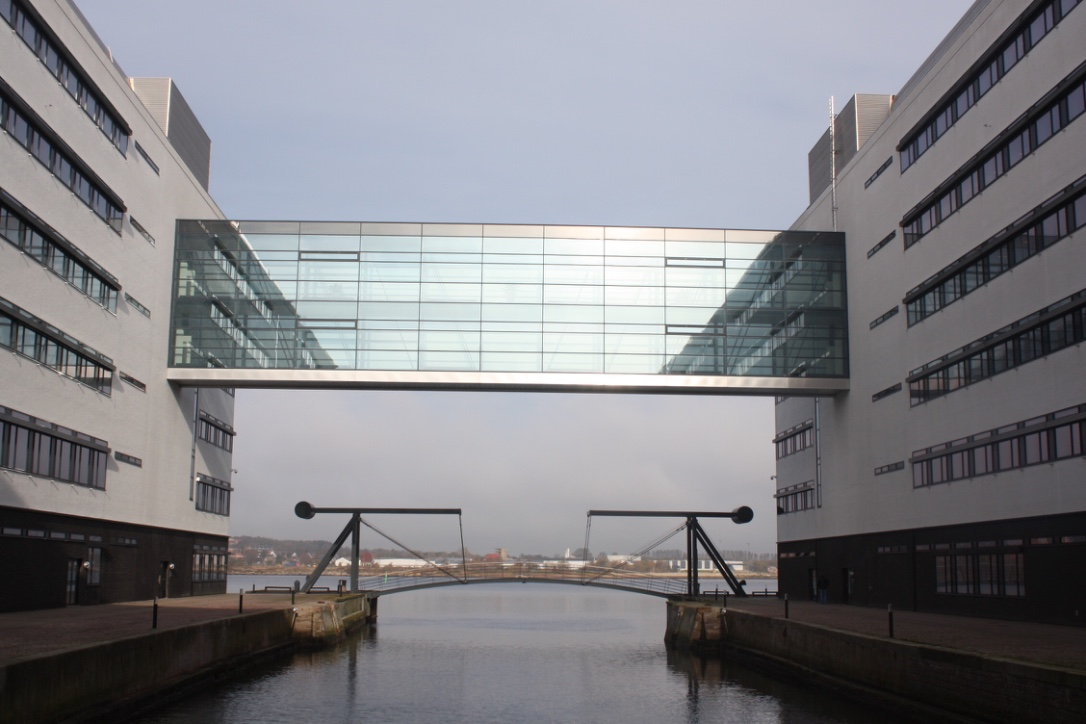
\includegraphics[width=1\textwidth]{billeder/KMDgangbro.jpg}

\vspace{2cm} 
\textsc{\Large P2 - Projekt \\
Gruppe B2-23 \\
Byggeri \& Anlæg 2\\
Aalborg Universitet\\
Den 23. maj 2016\\}
\end{flushright}

\cleardoublepage												% Indsaetter tom side, saa naeste kapitel starter paa hoejre side (hvis noedvendigt)
% Dette er LaTeX-versionen af titelbladet for TNB studenterrapporter
% Filen kræver:
% Universitetets logo:  AAU-logo-stud-UK eller AAU-logo-stud-DK
% Synopsis: En fil ved navn synopsis.tex

% Udarbejdet af: Jesper Nørgaard (jesper@noergaard.eu) 10. april 2012

\phantomsection
\pdfbookmark[0]{Titelblad}{titelblad}
\thispagestyle{empty}

\begin{minipage}[t]{0.48\textwidth}
\vspace*{-25pt}			%\vspace*{-9pt}

\includegraphics[height=4cm]{billeder/AAU-logo-stud-DK-RGB}
\end{minipage}
\hfill
\begin{minipage}[t]{0.48\textwidth}
{\small 
\textbf{Første Studieår v/ Det Teknisk-}\\
\textbf{Naturvidenskabelige Fakultet}  \\
Byggeri og Anlæg \\
Strandvejen 12-14 \\
9000 Aalborg \\
http://www.tnb.aau.dk}
\end{minipage}

\vspace*{1cm}

\begin{minipage}[t]{0.48\textwidth}
\textbf{Titel:} \\[5pt]\hspace{2ex}
Fundering af tilbygning af Strøybergs Palæ \bigskip

\textbf{Projekt:} \\[5pt]\bigskip\hspace{2ex}
P2-projekt

\textbf{Projektperiode:} \\[5pt]\bigskip\hspace{2ex}
Februar 2016 - maj 2016

\textbf{Projektgruppe:} \\[5pt]\bigskip\hspace{2ex}
B2-23	

\textbf{Deltagere:} \\[5pt]\hspace*{2ex}
Alexander Schacht \\\hspace*{2ex}
Emil Faber B.-S. \\\hspace*{2ex}
Hussein Al-Ali \\\hspace*{2ex}
Johnny Tuan N. \\\hspace*{2ex}
Jonas Damsbo \\\hspace*{2ex}
Mads Bjørndal N.\\\bigskip\hspace*{2ex}
Massir Thaafghan

\textbf{Vejledere:} \\[5pt]\hspace*{2ex}
Søren Dam Nielsen og Niels Agerholm




\vspace*{1cm}

\textbf{Oplagstal: 10} \\
\textbf{Sidetal: 118 } \\
\textbf{Appendiks: 33 } \\ 
\textbf{Afsluttet 18-12-2015}

\end{minipage}
\hfill
\begin{minipage}[t]{0.483\textwidth}
Synopsis: \\[5pt]
\fbox{\parbox{7cm}{\bigskipDette P1-projekt omhandler KMDs nordlige langt-spændende gangbro, som forbinder KMDs to hovedbygninger med hinanden. I kapitlet \textit{Beskrivelse af konstruktion}, beskrives KMDs gangbro detaljeret, med hvilke materialer den er lavet af samt dens dimensioner. I kapitlet \textit{Stål og dets egenskaber}, beskrives det anvendte stål, dets flydespænding samt dets tryk og træk styrker. I kapitlet \textit{Standarder og normer}, beskrives hvad Eurocodes, Dansk Standard, partialkoefficienter og Bygningsreglementet er. I kapitlet \textit{Laster} beregnes egen-, nyttelasten, vind- og snelasterne for KMDs gangbro. I kapitlet \textit{Statisk dokumentation} beregnes reaktionerne og de indre kræfter. Dernæst bevises det, at bæreevne er tilstrækkelig. Tilsidst konkluderes de opstillede problemstillinger i en besvarelse, hvor det munder ud i, at gangbroen er dimensioneret tilstrækkeligt.


\bigskip}}
\end{minipage}

\vfill

{\footnotesize\itshape Rapportens indhold er frit tilgængeligt, men offentliggørelse (med kildeangivelse) må kun ske efter aftale med forfatterne.}

% Rapportens indhold er frit tilgængeligt, men offentliggørelse (med kildeangivelse) må kun ske efter aftale med forfatterne.
% The content of the report is freely available, but publication (with source reference) may only take place in agreement with the authors.

\cleardoublepage
\chapter*{Forord}

Denne rapport er resultatet af det arbejde projektgruppen A408a, bachelor Byggeri og Anlæg på Aalborg Universitet, har lavet i P1-projektet på første semester. Rapporten er udarbejdet fra perioden d. 6. oktober til d. 18. december. Det overordnede emne for dette P1-projekt er; Aalborg, en by i stadig forandring, med underemnet; Analyse af bæreevnen af langt-spændende gangbro, hvor der er arbejdet med tekniske og kontekstuelle problemstillinger for udformningen af KMDs gangbro og eftervisning af dens bæreevne. Vi vil gerne takke vores vejleder, Jonas Bjerg Thomsen, for hans indsats, hjælp og gode samarbejde igennem hele projektperioden.

\textbf{Læsevejledning}

Rapporten udformet således, at der løbende kommer kildehenvisninger i teksten, som til sidst er uddybet i en litteraturliste. Kildehenvisningerne i denne rapport er lavet med Harvard metoden, som angives med: [Forfatterens efternavn/virksomhed, udgivelsesår]. Ved referering til en hjemmeside anvendes samme metode, dog skrives der i litteraturlisten hvornår den sidst blev set. I litteraturlisten er kilderne organiseret i en kronologisk rækkefølge. Hvis der er en kilde, som har samme forfatterefternavn og udgivelsesår, tilføjes et suffiks i form af et bogstav (a,b osv.), dette gøres, så det er muligt at kende forskel på kilderne. I selve litteraturlisten angives forfatter(e), titel, udgave, oplag, ISBN-nummer og forlag, hvor hjemmesider har forfatter(e) eller virksomhed, titel, internetadresse, årstal og besøgsdato. Figur- og tabel nummerering er opstillet i kronologisk rækkefølge. Det første tal i et figur- eller tabelnummer er kapitelnummeret, det andet tal er figurens eller tabellens navn. Et eksempel på dette kunne være den femte figur i kapitel tre, den vil blive nummeret som Figur 3.5. Figurer uden en kildehenvisning er udarbejdet af projektgruppen selv.



\phantom{Luft}

\phantom{Luft}

\begin{table}[H]
	\centering
		\begin{tabular}{c c c}
			\underline{\phantom{mmmmmmmmmmmmmm}} & \underline{\phantom{mmmmmmmmmmmmmm}} & \underline{\phantom{mmmmmmmmmmmmmm}} \\
			Alexander Schacht			& Emil Faber B.-S. 		& Hussein Al-Ali 			\\
			&&\\
			&&\\
			\underline{\phantom{mmmmmmmmmmmmmm}} & \underline{\phantom{mmmmmmmmmmmmmm}} & \underline{\phantom{mmmmmmmmmmmmmm}} \\
			Johnny Tuan N.			& Jonas Damsbo 		& Mads Bjørndal N. 	\\
			&&\\
			&&\\			
&\underline{\phantom{mmmmmmmmmmmmmm}} \\ 														
			& Massir Thaafghan
																		
		\end{tabular}
\end{table}
\cleardoublepage

%%%% Indholdsfortegnelse (TOC) %%%%

\phantomsection													% Kunstigt afsnit, som hyperlinks kan 'holde fast i'
\pdfbookmark[0]{Indholdsfortegnelse}{indhold}					% Tildeler en klikbar bookmark til den endelige PDF
\tableofcontents*												% Indholdsfortegnelsen (kaldet ToC) 

%\addtocontents{toc}{\protect\newpage}							% Fremtvinger sideskift i ToC hvis noedvendig (der hvor koden placeres)


\mainmatter														% Hovedindhold - nummereres fra side 1

%%%% Rapportindhold %%%% 										% Rapportindholdet boer IKKE indeholde broedtekst - KUN includede filer!

%% Indledende %%												% Opdel evt. i passende afsnit for overblikkets skyld

\chapter{Indledning}



\chapter{Problemanalyse}
Dette afsnit vil indeholde en argumentation for, hvad denne rapports grundlæggende emnevalg er samt en motivationsdel til rapporten, som er givet ud fra en undren over emnet. Til sidst vil metodevalget blive begrundet.  
 
\section{Initierende problem}
KMDs langt-spændende gangbro er en konstruktion, der er udformet som en gitterkonstruktion. Dette danner grundlag for en gennemgang af analytiske modeller og metoder, der anvendes til at bestemme konstruktionens stabilitet og dimensioner. Igennem tiderne har forkerte modeller og metoder betydet delvise eller totale kollaps for bygninger. For eksempel da Superarenaen i Ballerup kollapsede den 3. januar 2003  pga. fejldimensionering af bjælkerne og i vinteren 2009-2010 hvor der skete en sammenstyrtning af en stald pga. en dimensioneringsfejl i de bærende søjler. I dette projekt vil der forsøges at opnå en forståelse af de anvendte modeller og metoder til at eftervise en konstruktions bæreevne og hvordan den er sikret via beregningerne. Dette rejser en række interessante spørgsmål, som er opdelt i følgende punktform. 
 
 \begin{itemize}
 \item Hvad påvirker gangbroens konstruktion?
 \item Hvilke metoder anvendes ved bestemmelse af bæreevnen? 
 \item Hvordan sikres konstruktionerne i de benyttede last- og beregningsmodeller? 
 \end{itemize}
 
\section{Problemformulering}
Ved den initierende problemstilling blev der set på nogle interessante områder, som projektgruppen ønsker at eftervise med denne rapport. Dette munder ud i en konkret problemstilling, hvor metoden last-system-respons vil være oplagt at anvende til beregning eller eftervisning af konstruktionens stabilitet og dimensioner. Dette sikrer processen fra modeller og forudsætninger til virkeligheden. For at man nemmere kan tyde de opstillede problemer, opdeles det i følgende underpunkter.

\begin{itemize}
\item Hvilken type konstruktion er KMDs gangbro?
\item Hvorfor er stål egnet som byggemateriale?
\item Hvilke laster bliver gangbroen påvirket af?
\item Hvordan anvendes knudepunktsmetoden til at finde den samlede lastpåvirkning for gangbroen?
\item Er dimensionerne af profilerne i gangbroen tilstrækkelige?
\end{itemize}

\section{Problemafgrænsning}
I denne rapport er projektets fokus, hvilket grundlag der er for dimensioneringen af gangbroen. Dette munder ud i en statisk model, som består af relevante beregninger, som resulterer i hvorvidt dimensioneringen af stålprofiler er korrekt eller i så fald er overdimensioneret eller underdimensioneret. Igennem rapporten vil de relevante metoder blive brugt til at besvare problemstillingerne. Rapporten er udarbejdet, som et produkt af et P1-projekt indenfor det ingeniørvidenskabelige basisår. Dette resulterer i en tidsbegrænset proces, som har betydning for rapportens indhold og derfor er det nødvendigt at lave en afgræsning. Derfor vil nedenstående problemstillinger ikke blive taget i betragtning og vil dermed blive afgrænset fra rapporten:

\begin{itemize}
\item KMDs to hovedbygninger.
\item Aalborgs lokalplan for Sturhs Brygge.
\item Geotekniks analyse af byggegrunden. 
\item Det økonomiske aspekt indenfor byggeprojektet.
\item Gangbroens energi og indeklima.
\item KMDs begrundelse for opførelsen af gangbroen.
\item De indre vindkræfter.
\item De arkitektoniske overvejelser. 
\item De hensigtsmæssige ulykkeslaster og brandsikringen.
\end{itemize}

\section{Metodevalg}
P1-projektets metodevalg er baseret på, at rapporten vil beskrive KMDs gangbro ud fra en ingeniørs synsvinkel. Metoden behandler tre hovedpunkter, som kendes fra én metode, last-system-responsmetoden. Denne metode anvendes til overvejelser for gangbroens konstruktion. Projektet vil inddrage beregninger, som vedrører de forskellige laster. Det, som optager lasterne er gangbroens konstruktion, hvormed gitterkonstruktionen er systemet, som håndterer lasterne.  Responsen af gangbroen er herefter det interessante, hvor det kan sættes i sammenhæng med, om konstruktionen er tilstrækkelig dimensioneret. Der vil blive analyseret ud fra beregninger af de indre kræfter i gangbroen.




\chapter{Konklusion}
Denne rapport dokumenterer, at den nordlige gangbro ved KMD er konstrueret korrekt i form af tilstrækkelig bæreevne i forhold til de forskellige laster, som den bliver udsat for. 

Ud fra rapporten konkluderes der, at KMDs gangbro er en konstruktion, der er konstrueret som en gitterkonstruktion. En gitterkonstruktion er en konstruktion, som er opbygget af stænger, som udgør trekanter. Konstruktionen er opbygget som en statisk ubestemt konstruktion, men for at gøre det muligt at beregne de indre kræfter, ved hjælp af knudepunktsmetoden i konstruktionen, er der indsat en fiktiv stang for at gøre konstruktionen statisk bestemt.  

Stål er et velegnet materiale til gangbroen, da stål har en meget høj trækstyrke, hvilket underflangen af gangbroen vil blive udsat for. En anden grund til, at stål er et velegnet byggemateriale er, at det kan fremstilles i en lang række forskellige kvaliteter, alt efter hvilken opgave det skal have.

I denne rapport er der blevet beregnet på fire forskellige laster, som påvirker KMDs gangbro; egen-, nytte-, vind- og snelast. De forskellige laster er blevet ført ud på 48 forskellige knudepunkter. Egenlasten er den last, som en konstruktion belaster sig selv med og er blevet beregnet ud fra de materialer gangbroen er bygget af. Nyttelasten er den last, som gangbroen udsættes for af mennesker og inventar. Nyttelasten er beregnet ud fra en standard, som passer til gangbroens kategori i forhold til hvad den anvendes til. Vindlast er den last, som vinden påvirker en konstruktion med. Vindlasten er beregnet ud fra en række standarder og normer, fundet i Eurocodes, såsom hvor høj en konstruktion er, hvilket område konstruktionen ligger i, om der står andre konstruktioner i nærheden og hvor i landet konstruktionen ligger. Vindlasten er den eneste last, der i denne rapport både påvirker det vertikale og horisontale gitter. Snelasten er den last, som sne påvirker en konstruktion med, den virker udelukkende på taget af KMDs gangbro og den kan både være jævnt og ujævnt fordelt derpå. Snelasten beregnes også ud fra information, der fås i Eurocode og ud fra, at der forekommer snedriver når konstruktionen ligger imellem to højere konstruktioner, som er tilfældet for KMDs gangbro. 

Ud fra egen-, nytte-, vind- og snelasterne er der blevet beregnet lastkombinationer hvor de forskellige laster på skift er beregnet som dominerende. Der bliver ganget partialkoefficienter på lastkombinationerne for at sørge for, at lasterne bliver overvurderet i forhold til hvor store de er i den virkelige verden. Dette gøres for at sikre en mindre risiko for kollaps, da modeller og virkelighed ikke altid stemmer overens. Laster hvor partialkoefficienter er multipliceret på kaldes regningsmæssige laster. Den største regningsmæssige last bliver herefter anvendt til eftervisning af bæreevnen. På KMDs gangbro er det den lastkombination, hvor nyttelasten er dominerende, der er størst. 


Med viden om, at gangbroen er statisk bestemt, er stangkræfterne beregnet ved anvendelse af knudepunktsmetoden. Ved brug af knudepunktsmetoden løsskæres alle knudepunkter fra hinanden og der beregnes horisontal og vertikal ligevægt for indre kræfter ved knudepunkter.  Ved beregningerne af stangkræfterne bliver det fastlagt hvilke stænger der er træk- eller trykstænger. Ud fra de beregnede indre kræfter, er der opstillet en statisk model, som efterviser, at den regningsmæssige spænding er lavere end profilens maksimale tilladte spænding.  

Ud fra den statiske dokumentation kan det konkluderes, at de regningsmæssige spændinger i profilerne er mindre end den tilladte spænding, derfor er gangbroen dimensioneret tilstrækkeligt, ud fra de antagelser der er lavet i rapporten. Den fiktive stang der blev placeret for at kunne anvende knudepunktsmetoden, og ud fra beregningen af de indre kræfter kan det konkluderes, at den fiktive stang er minimalt belastet.  

%\chapter{Konklusion}
Denne rapport dokumenterer, at den nordlige gangbro ved KMD er konstrueret korrekt i form af tilstrækkelig bæreevne i forhold til de forskellige laster, som den bliver udsat for. 

Ud fra rapporten konkluderes der, at KMDs gangbro er en konstruktion, der er konstrueret som en gitterkonstruktion. En gitterkonstruktion er en konstruktion, som er opbygget af stænger, som udgør trekanter. Konstruktionen er opbygget som en statisk ubestemt konstruktion, men for at gøre det muligt at beregne de indre kræfter, ved hjælp af knudepunktsmetoden i konstruktionen, er der indsat en fiktiv stang for at gøre konstruktionen statisk bestemt.  

Stål er et velegnet materiale til gangbroen, da stål har en meget høj trækstyrke, hvilket underflangen af gangbroen vil blive udsat for. En anden grund til, at stål er et velegnet byggemateriale er, at det kan fremstilles i en lang række forskellige kvaliteter, alt efter hvilken opgave det skal have.

I denne rapport er der blevet beregnet på fire forskellige laster, som påvirker KMDs gangbro; egen-, nytte-, vind- og snelast. De forskellige laster er blevet ført ud på 48 forskellige knudepunkter. Egenlasten er den last, som en konstruktion belaster sig selv med og er blevet beregnet ud fra de materialer gangbroen er bygget af. Nyttelasten er den last, som gangbroen udsættes for af mennesker og inventar. Nyttelasten er beregnet ud fra en standard, som passer til gangbroens kategori i forhold til hvad den anvendes til. Vindlast er den last, som vinden påvirker en konstruktion med. Vindlasten er beregnet ud fra en række standarder og normer, fundet i Eurocodes, såsom hvor høj en konstruktion er, hvilket område konstruktionen ligger i, om der står andre konstruktioner i nærheden og hvor i landet konstruktionen ligger. Vindlasten er den eneste last, der i denne rapport både påvirker det vertikale og horisontale gitter. Snelasten er den last, som sne påvirker en konstruktion med, den virker udelukkende på taget af KMDs gangbro og den kan både være jævnt og ujævnt fordelt derpå. Snelasten beregnes også ud fra information, der fås i Eurocode og ud fra, at der forekommer snedriver når konstruktionen ligger imellem to højere konstruktioner, som er tilfældet for KMDs gangbro. 

Ud fra egen-, nytte-, vind- og snelasterne er der blevet beregnet lastkombinationer hvor de forskellige laster på skift er beregnet som dominerende. Der bliver ganget partialkoefficienter på lastkombinationerne for at sørge for, at lasterne bliver overvurderet i forhold til hvor store de er i den virkelige verden. Dette gøres for at sikre en mindre risiko for kollaps, da modeller og virkelighed ikke altid stemmer overens. Laster hvor partialkoefficienter er multipliceret på kaldes regningsmæssige laster. Den største regningsmæssige last bliver herefter anvendt til eftervisning af bæreevnen. På KMDs gangbro er det den lastkombination, hvor nyttelasten er dominerende, der er størst. 


Med viden om, at gangbroen er statisk bestemt, er stangkræfterne beregnet ved anvendelse af knudepunktsmetoden. Ved brug af knudepunktsmetoden løsskæres alle knudepunkter fra hinanden og der beregnes horisontal og vertikal ligevægt for indre kræfter ved knudepunkter.  Ved beregningerne af stangkræfterne bliver det fastlagt hvilke stænger der er træk- eller trykstænger. Ud fra de beregnede indre kræfter, er der opstillet en statisk model, som efterviser, at den regningsmæssige spænding er lavere end profilens maksimale tilladte spænding.  

Ud fra den statiske dokumentation kan det konkluderes, at de regningsmæssige spændinger i profilerne er mindre end den tilladte spænding, derfor er gangbroen dimensioneret tilstrækkeligt, ud fra de antagelser der er lavet i rapporten. Den fiktive stang der blev placeret for at kunne anvende knudepunktsmetoden, og ud fra beregningen af de indre kræfter kan det konkluderes, at den fiktive stang er minimalt belastet.  



%%%% Kilder %%%%


\begingroup
	\raggedright
	\bibliography{bibtex/litteratur}						% Litteraturlisten inkluderes
\endgroup

%%%% Fixme-listen %%%%

\newpage														% Ny side til Fixme-listen
%\listoffixmes													% Fixme-listen - fjernes til sidst i projektet med "%"


%%%% Appendiks %%%%

\appendix
\clearforchapter												% Sikrer at pagestylen aktiveres paa den rigtige side
\phantomsection													% Kunstigt afsnit, som hyperlinks kan 'holde fast i'
\pdfbookmark[0]{Appendiks}{appendiks}							% Tildeler en klikbar bookmark til den endelige PDF

%% Indstillinger for appendiks (deaktiveret med "%") %%

%\pagestyle{empty}												% Sidehoved/-fod for standardsider aendres til tom for appendiks
%\aliaspagestyle{chapter}{empty}								% Sidehoved/-fod for kapitelsider aendres til tom for appendiks
%\settocdepth{chapter}											% Kun kapitel-niveau vises i ToC
%\addtocontents{toc}{\protect\cftpagenumbersoff{chapter}}		% Sidetal for kapitler fjernes i ToC

%% Filer til appendiks %%

														% Appendiks/bilag start - giver chapter bogstaver i stedet for tal
%\input{appendiks/appendiks2}
%%%% Bilag %%%%

%\phantomsection												% Kunstigt afsnit, som hyperlinks kan 'holde fast i'
%\addcontentsline{toc}{chapter}{Bilag A \ Navn} 				% Manuelle indgange i indholdsfortegnelsen (naar \includepdf bruges)

%\includepdf[pages={x-y}]{filnavn}								% Inkluder eksterne bilag med \includepdf[pages={x-y}]{filnavn}


\end{document}													% Slutter dokumentet - obligatorisk


